\begin{abcliste}
\abc Skizze (Neigung übertrieben gezeichnet):
\begin{center}
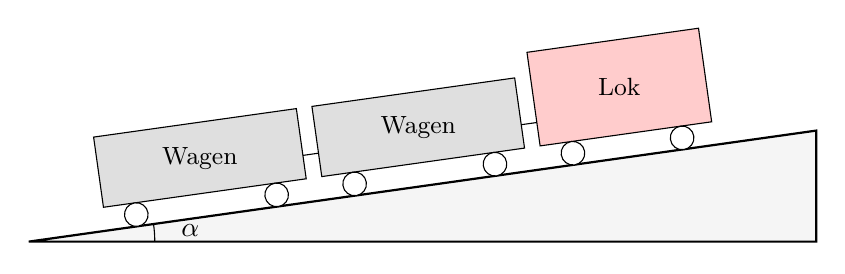
\begin{tikzpicture}[>=stealth]
 \draw[thick, fill=gray!8] (0,0) -- (10,0) -- (10,1.41) -- cycle;
 \draw (1.6,0) arc (0:8:1.6);
 \node at (2.05,0.14) {$\alpha$};
 \begin{scope}[rotate=8]
  \draw[fill=gray!25] (1.0,0.3) rectangle (3.6,1.2);
  \draw[fill=gray!25] (3.8,0.3) rectangle (6.4,1.2);
  \draw[fill=red!20] (6.6,0.3) rectangle (8.8,1.5);
  \draw (3.6,0.6) -- (3.8,0.6) (6.4,0.6) -- (6.6,0.6);
  \foreach \x in {1.4,3.2,4.2,6.0,7.0,8.4} \draw[fill=white] (\x,0.15) circle (0.15);
  \node[font=\small] at (2.3,0.75) {Wagen};
  \node[font=\small] at (5.1,0.75) {Wagen};
  \node[font=\small] at (7.7,0.9) {Lok};
 \end{scope}
\end{tikzpicture}
\end{center}
Kräfteplan für die ganze Komposition (oben) und für die Lokomotive allein (unten), bei gleichmässiger Fahrt und ohne Reibung, nicht massstäblich:
\begin{center}
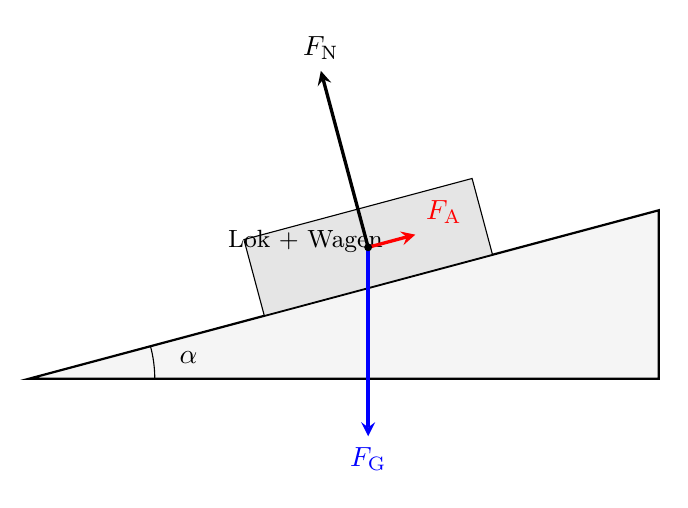
\begin{tikzpicture}[>=stealth]
 \draw[thick, fill=gray!8] (0,0) -- (8.00,0) -- (8.00,2.14) -- cycle;
 \draw (1.6,0) arc (0:15:1.6);
 \node at (2.03,0.27) {$\alpha$};
 \begin{scope}[shift={(4.44,1.19)}, rotate=15]
  \draw[fill=gray!20] (-1.5,0) rectangle (1.5,1.0);
  \node[font=\small] at (-0.75,0.78) {Lok + Wagen};
 \end{scope}
 \draw[->, very thick, blue] (4.31,1.67) -- ++(-90.00:2.40) node[anchor=north] {$F_\mathrm{G}$};
 \draw[->, very thick, black] (4.31,1.67) -- ++(105.00:2.32) node[anchor=south] {$F_\mathrm{N}$};
 \draw[->, very thick, red] (4.31,1.67) -- ++(15.00:0.62) node[anchor=south west] {$F_\mathrm{A}$};
 \fill (4.31,1.67) circle (0.05);
\end{tikzpicture}
\end{center}
\begin{center}
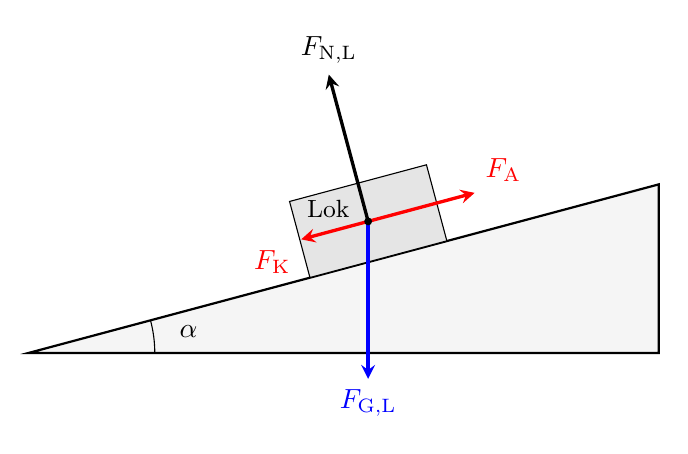
\begin{tikzpicture}[>=stealth]
 \draw[thick, fill=gray!8] (0,0) -- (8.00,0) -- (8.00,2.14) -- cycle;
 \draw (1.6,0) arc (0:15:1.6);
 \node at (2.03,0.27) {$\alpha$};
 \begin{scope}[shift={(4.44,1.19)}, rotate=15]
  \draw[fill=gray!20] (-0.9,0) rectangle (0.9,1.0);
  \node[font=\small] at (-0.45,0.78) {Lok};
 \end{scope}
 \draw[->, very thick, blue] (4.31,1.67) -- ++(-90.00:2.00) node[anchor=north] {$F_\mathrm{G,L}$};
 \draw[->, very thick, black] (4.31,1.67) -- ++(105.00:1.93) node[anchor=south] {$F_\mathrm{N,L}$};
 \draw[->, very thick, red] (4.31,1.67) -- ++(15.00:1.40) node[anchor=south west] {$F_\mathrm{A}$};
 \draw[->, very thick, red] (4.31,1.67) -- ++(195.00:0.88) node[anchor=north east] {$F_\mathrm{K}$};
 \fill (4.31,1.67) circle (0.05);
\end{tikzpicture}
\end{center}
Auf die ganze Komposition wirken die Gewichtskraft $F_\mathrm{G}$, die Normalkraft $F_\mathrm{N}$ der Schienen und die Antriebskraft $F_\mathrm{A}$, die als Haftreibungskraft der Schienen an den Rädern der Lokomotive angreift. Auf die Lokomotive allein wirken ihre Gewichtskraft $F_\mathrm{G,L}$, ihre Normalkraft $F_\mathrm{N,L}$, die Antriebskraft $F_\mathrm{A}$ und die Kraft $F_\mathrm{K}$, mit der die Wagen über die Kupplung hangabwärts an ihr ziehen. Die Kupplungskraft ist für die ganze Komposition eine innere Kraft und erscheint deshalb nur im zweiten Kräfteplan.

\abc Rollt die Komposition reibungsfrei talwärts, beschleunigt sie die Hangabtriebskraft $\left(m_\mathrm{L}+m_\mathrm{Z}\right)g\sin\alpha$. Die Masse fällt heraus:
\begin{align}
 a &= \aTaF = \gE\cdot\sin\left(\wiO\right) = \aTa \approx \result{\aTaP{0}{2}}
\end{align}
Bei gleichmässiger Fahrt ist die resultierende Kraft auf die Wagen null. Die Lokomotive muss sie also mit der Hangabtriebskraft der Wagen ziehen:
\begin{align}
 F_\mathrm{K} &= \FKuF \\
   &= \mZu\cdot\gE\cdot\sin\left(\wiO\right) \\
   &= \FKu \approx \result{\FKuP{3}{2}}
\end{align}
Die Antriebskraft der Schienen auf die Lokomotive ist grösser, sie muss auch die Lokomotive selbst hinaufziehen: $F_\mathrm{A} = \FAnF = \FAnP{3}{2}$.
\end{abcliste}
